\documentclass{article}%
\usepackage[T1]{fontenc}%
\usepackage[utf8]{inputenc}%
\usepackage{lmodern}%
\usepackage{textcomp}%
\usepackage{lastpage}%
\usepackage{authblk}%
\usepackage{graphicx}%
%
\title{Interplay of RsbM and RsbK controls the sB activity of Bacillus cereuse}%
\author{Diamond Adams}%
\affil{Oncology Research, Pfizer Worldwide Research and Development, San Diego, California, United States of America}%
\date{01{-}01{-}2013}%
%
\begin{document}%
\normalsize%
\maketitle%
\section{Abstract}%
\label{sec:Abstract}%
If you've played video games over the past year, then chances are that you've encountered X{-}Box Binding Protein 1 (XBP1s). The XBP1s are rare forms of streptococcus pneumonia that are found in infants. If you're interested in finding out what can happen to an infant exposed to XBP1s, let me introduce you to a researcher in the Center for the Prevention of Infectious Diseases at the William Beaumont Army Medical Center.\newline%
This video from the Center for the Prevention of Infectious Diseases about XBP1s describes the protein structure. It begins by stating that XBP1s is "an antibacterial source{-}control protein found in a lot of viral infection cultures." This type of research could conceivably transform the way scientists learn about streptococcus infections in humans. The video goes on to explain the protein's role in regulating pathogens, including those that can cause tuberculosis, typhoid, and pneumonia. In short, XBP1s are a key element of the pathogen.\newline%
Here's the problem. We don't know much about XBP1s in humans, except how it interacts with other proteins in one's body. A key study in the New England Journal of Medicine noted that XBP1, when consumed orally, "contains many more or fewer cytoplasmic proteases than do protease{-}negative proclamations expressed by the Bacteroides family of bacterial compounds." Yup, XBP1's role in infectious disease is known, but there's a lot we don't know about how it interacts with other proteins in our bodies. And so it follows that XBP1 has now been identified as a key input into infectious disease progression in humans.\newline%
The Centers for Disease Control and Prevention has shown that XBP1s have important functions in all the host{-}borne infections that the agency detects. It is, in the summary, one of "a number of viral infections directly associated with pneumonia and tuberculosis" and "as a result of the presence of XBP1s, these organisms have been identified as some of the principal pathogens that cause many human infectious diseases." We now know how to keep the XBP1s from invading the entire human host. It's as simple as that.\newline%
A recent paper by researchers at the University of Washington, Instituto de la Reina de La Ra HIDTA and SFRIF (RIV Certo de apoio humanitara do Literalnava) presented in the December 2013 issue of Global Infectious Diseases concludes that its uses in human diseases may be even more important than previous ideas. Dr. Maria Isabel Gonzalez{-}Paesi, PhD, from the research laboratory of Professor Lozano Machado, adds that XBP1 can become "a very important defense mechanism against streptococcus, myocardial infarction, and other infections."\newline%
If you're looking for more information about XBP1s, in particular the potential benefits for infants exposed to XBP1s, you'll find it in a forthcoming paper at Vaccinexpert.com. The authors describe a study in Peru of an infant exposed to XBP1s. It's important to note that XBP1 is currently being used by the CDC for the population{-}wide clinical surveillance programs where babies are routinely checked for signs of strep. But if XBP1 can be developed into a real indicator that an infant has strep in his or her body, that will likely be a good thing.

%
\subsection{Image Analysis}%
\label{subsec:ImageAnalysis}%


\begin{figure}[h!]%
\centering%
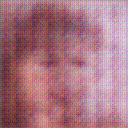
\includegraphics[width=150px]{500_fake_images/samples_5_133.png}%
\caption{A Black And White Photo Of A Black And White Background}%
\end{figure}

%
\end{document}